%----------Required Packages----------
\documentclass[12pt]{article}
\usepackage[maxauthors=10,articletitle=true]{achemso}
\usepackage[version=4]{mhchem}
\usepackage[scale=0.80]{geometry}
\usepackage[utf8]{inputenc}
\usepackage{amsmath, amssymb, amsfonts}
\usepackage{multirow}
\usepackage{booktabs}
\usepackage{makecell}
\usepackage{setspace}
\usepackage{rotating}
\usepackage{titlesec}
\usepackage{caption}
\usepackage[linktocpage,colorlinks=true,linkcolor=black,urlcolor=black,
citecolor=black,hyperfigures]{hyperref}
\usepackage{graphicx}
\usepackage{float}
\usepackage{threeparttable}
\usepackage{setspace}
\usepackage[numbib,nottoc]{tocbibind}
\usepackage{color, colortbl}
\usepackage{enumerate}
\usepackage[table]{xcolor}
\usepackage{natbib}
\usepackage{authblk} % For multiple authors and affiliations
\renewcommand{\thepage}{S\arabic{page}}
\setcounter{page}{1}                  

\newcommand{\cob}{\color{blue}}
\newcommand{\com}{\color{magenta}}
\newcommand{\voc}{$V_\mathrm{OC}$}
\newcommand{\jsc}{$J_\mathrm{SC}$}
\newcommand{\pce}{PCE$_\mathrm{{max}}$}
\newcommand{\eb}{$E_\mathrm{b}$}
\newcommand{\ex}{$E_\mathrm{x}$}
\newcommand{\gs}{S$_0$}
\newcommand{\sing}{S$_1$}
\newcommand{\lamb}{$\lambda_\mathrm{max}$}
\newcommand{\delGCR}{$\Delta G_\mathrm{CR}$}
\newcommand{\delGCS}{$\Delta G_\mathrm{CS}$}
\newcommand{\delGCT}{$\Delta G_\mathrm{CT}$}
\newcommand{\kCR}{$k_\mathrm{CR}$}
\newcommand{\kCS}{$k_\mathrm{CS}$}
\newcommand{\Eloss}{$E_\mathrm{loss}$}
\newcommand{\delmu}{$\Delta \mu$}
\newcommand{\ehl}{$\Delta E_\mathrm{HOMO-LUMO}$}
\newcommand{\qpole}{$Q_\mathrm{20}$}
\newcommand{\maxl}{$\lambda_\mathrm{max}$}
\newcommand{\dlumo}{$\Delta E_\mathrm{LUMO}$}


\newcommand{\planeang}{$\theta_\mathrm{plane}$}
\newcommand{\backang}{$\theta_\mathrm{bb}$}
\newcommand{\erep}{$\Delta E_\mathrm{xrep}$}
\newcommand{\silscore}{$S_\mathrm{sil}$}
\newcommand{\freevol}{$V_\mathrm{free}$}
\newcommand{\meandist}{$r_\mathrm{DA}$}

%----------Title Section----------
\makeatletter
\renewcommand{\maketitle}{
\begin{center}
{\LARGE \textbf{\@title}} \\[1em]   % Title font size and style
{\large \@author} \\[1em]           % Author font size
{\small \@date}                     % Date font size
\end{center}
}
\makeatother

%----------Useful commands----------
\renewcommand{\arraystretch}{1.5}
\renewcommand\bibname{References}

\renewcommand{\thesection}{S\arabic{section}}
\renewcommand{\theequation}{S\arabic{equation}}
\renewcommand{\thefigure}{S\arabic{figure}}
\renewcommand{\thetable}{S\arabic{table}}

\setstretch{1.75}

%----------Page layout----------
\geometry{a4paper, margin=1in}
\onehalfspacing

%----------Section formatting----------
\titleformat{\section}{\large\bfseries}{\thesection}{1em}{}
\titleformat{\subsection}{\normalsize\bfseries}{\thesubsection}{1em}{}

%----------Custom Commands----------

\newcommand{\keywords}[1]{\textbf{Keywords:} #1}

%----------Title and Authors----------
\title{Supporting Information: \\ Synthesizability-Aware Hybrid Generative Workflow for Donor--Acceptor Discovery in Organic Photovoltaics}

\author[1,*]{Bibhas Das}
\author[1,*]{Anirban Mondal}

\affil[1]{\small Department of Chemistry, Indian Institute of Technology Gandhinagar, Gujarat, 382355, India}

\date{\small\today\\ {E-mail: dasbibhas@iitgn.ac.in, amondal@iitgn.ac.in}}

%----------------------------------------

\begin{document}
\maketitle
\clearpage

\section{Supporting Information: Computational Methods}
\subsection{Neural Component Implementation and Adversarial Training}
Neural components were implemented with TensorFlow/Keras 
\cite{abadi2016tensorflow} when the requisite training representation and valid training population were available. The coordinate-based adversarial component was trained separately for donor and acceptor populations, thereby avoiding the direct mixing of the two chemically distinct molecular classes. Trainable auxiliary components were tuned only where their architecture and validation data justified optimization; hyperparameter searches were conducted using Optuna 
\cite{akiba2019optuna}.

For the adversarial components, the discriminator and generator losses, along with the discriminator classification accuracy, were monitored at every training epoch. Under the standard binary minimax formulation, a balanced adversarial state is expected to approach $\mathcal{L}_{D}=\mathcal{L}_{G}=\ln 2 \approx 0.693$ with discriminator accuracy near $50\%$. Training was conducted over five epochs and 
monitored using a discriminator-loss safeguard of $\mathcal{L}_{D}<0.45$ to identify persistent discriminator dominance. This operational threshold was chosen as an early-warning level below the balanced minimax expectation, at which a persistently lower discriminator loss indicates that the discriminator is separating real and generated samples too easily \cite{goodfellow2014generative}. To reduce this risk, discriminator learning was attenuated relative to generator learning, discriminator updates were throttled after sustained domination, and the retained generator checkpoint was selected by proximity to the $\ln 2$ equilibrium rather than by the final epoch alone \cite{salimans2016improved}. This criterion was used to select a balanced training state and to avoid continued optimization once the discriminator became disproportionately stronger than the generator.

\subsection{Output Recording and Library-Level Reporting}
For every accepted molecule, the recorded information included its canonical structure, donor or acceptor class, proposal provenance, molecular novelty status, nearest-neighbor similarity, and synthetic-practicality indicators. For every evaluated donor--acceptor pair, the workflow retained the predicted values for the four device properties, the energy-loss quality-control estimate when available, the pair-level compatibility score, and the ranking information required to trace why the pair was selected for downstream assessment. Maintaining separate molecular- and pair-level records enables distinguishing a promising individual building block from a promising device combination.

The final libraries contained 52{,}995 donor candidates and 53{,}719 acceptor candidates after filtering for validity, exact novelty, duplicates, and near-neighbors. The pair-level screening analysis was conducted across 11{,}988{,}459 generated donor--acceptor combinations. These populations represent the chemically valid and nonredundant outputs of the computational filtering and combinatorial-screening protocol, not a count of experimentally synthesized molecules. Approach-level counts and rejection reasons were retained so that a high apparent output count cannot obscure a low valid-generation rate for a particular proposal route.

\subsection{Generative Quality Metrics}
Generation quality was quantified after the common filtering protocol. Validity was defined as the fraction of proposed structures that passed chemical sanitization and single-component checks; exact novelty as the fraction of retained structures absent from the relevant training library; and uniqueness after canonical duplicate removal. Internal diversity was calculated from pairwise Morgan-fingerprint similarities as
\begin{equation}
\mathrm{IntDiv}=1-\frac{2}{n(n-1)}\sum_{i<j}T_{ij},
\end{equation}
where $n$ is the number of molecules in the evaluated population and $T_{ij}$ is the Tanimoto similarity between molecules $i$ and $j$. This definition follows the MOSES convention \cite{moses}. Scaffold diversity was evaluated independently of fingerprint diversity because a library may exhibit diverse substituents while remaining concentrated in a small number of core structural families. The distance to the nearest training neighbor was also reported to complement exact novelty with a continuous measure of structural separation.

\subsection{Distribution-Level Distance Measures}
For detailed molecular-library characterization, a reproducible sample of 20{,}000 molecules from each molecular class was analyzed. Three distinct distribution-level distances were calculated: a fingerprint-based Fr\'echet distance derived from a low-dimensional projection of Morgan fingerprints, a property-embedding Fr\'echet distance obtained in the latent representation of an OPV-relevant property-prediction model, and the Fr\'echet ChemNet distance calculated in the published ChemNet embedding \cite{fcd}. These distances were retained as distinct quantities because they are defined in different embedding spaces and are not directly interchangeable. The ChemNet distance was reported only when molecular strings fell within the maximum input length accepted by its encoder. All generative metrics were calculated after the preceding validity and novelty filters to prevent invalid strings, duplicate structures, or exact training molecules from artificially inflating or deflating the assessment of the final candidate chemistry.

\subsection{Computational Partitioning and Reproducibility}
Computational tasks were partitioned across available workers for large-scale generation and screening, and all partitioned outputs underwent the same canonicalization and final duplicate checks before aggregation. Stage-specific records documented input counts, rejected structures, accepted molecules, model-selection statistics, and final pair-ranking summaries. Random seeds, software versions, model settings, curated input records, generated canonical structures, and out-of-fold prediction records are archived with the manuscript to permit independent reproduction and audit of the reported workflow.


\begin{figure}[!htb]
\centering
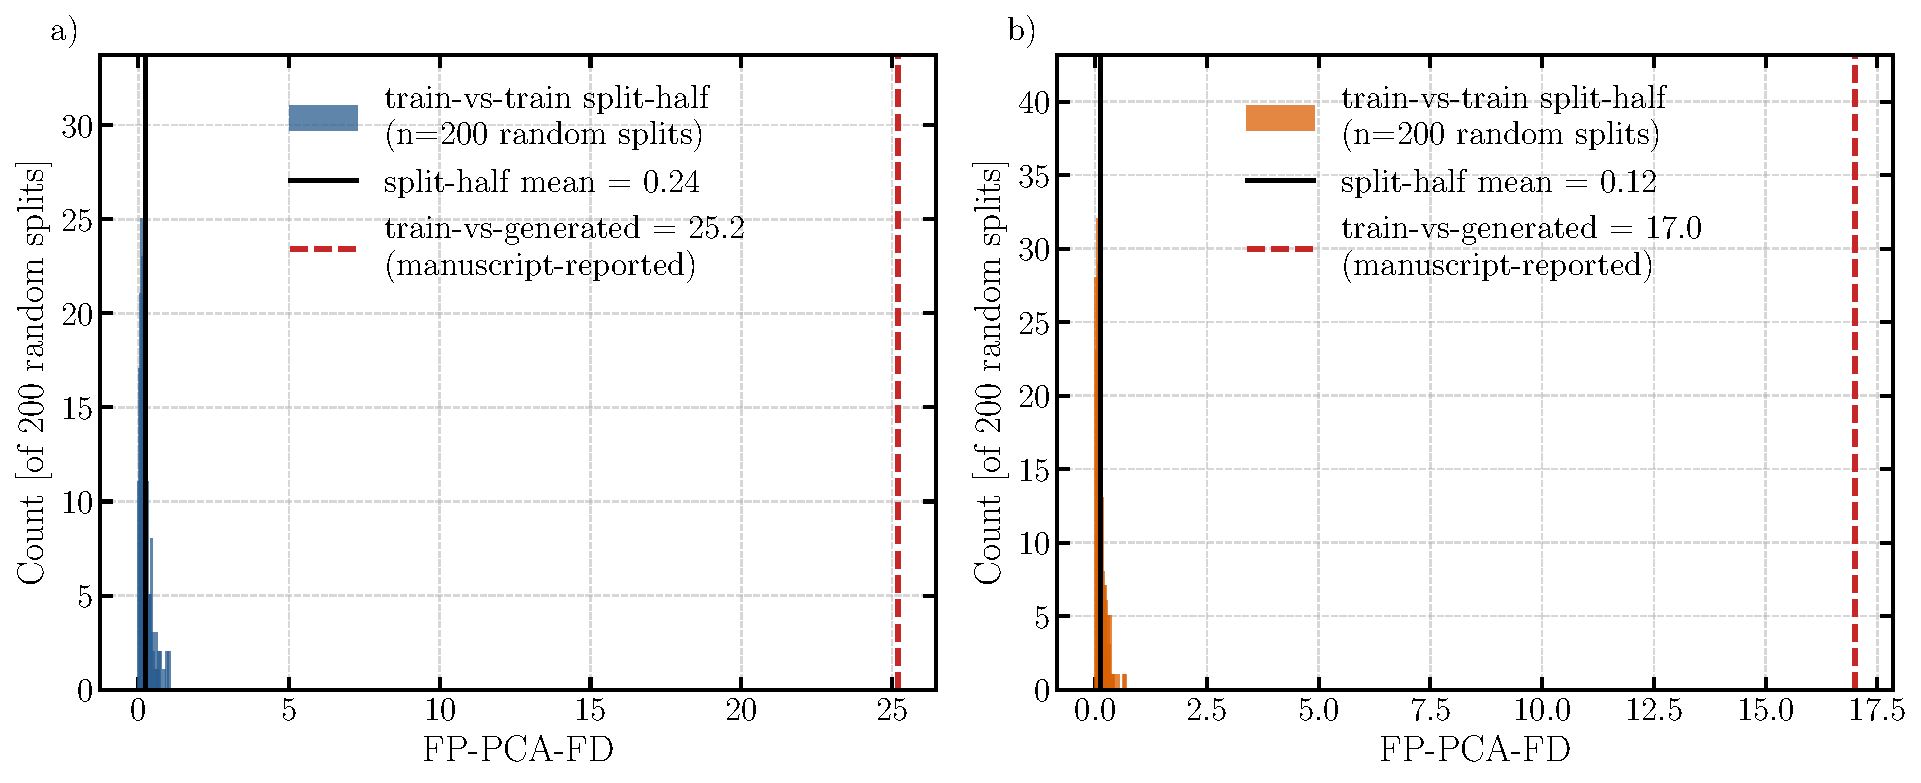
\includegraphics[width=15 cm]{figures/frechet_baseline_plot.pdf}
\caption{Train--train split-half null distribution of the fingerprint-space Fréchet distance (FP-PCA-FD) for the a) donor and b) acceptor reference libraries, obtained from 200 independent random 50/50 splits of each library against itself. The dashed red line marks the train-vs-generated FP-PCA-FD value reported in the main text ($25.2$ for donors, $17.0$ for acceptors), which lies far outside the split-half noise floor for both libraries.}
\label{fig:frechet_baseline}
\end{figure}

\begin{figure}[!htb]
\centering
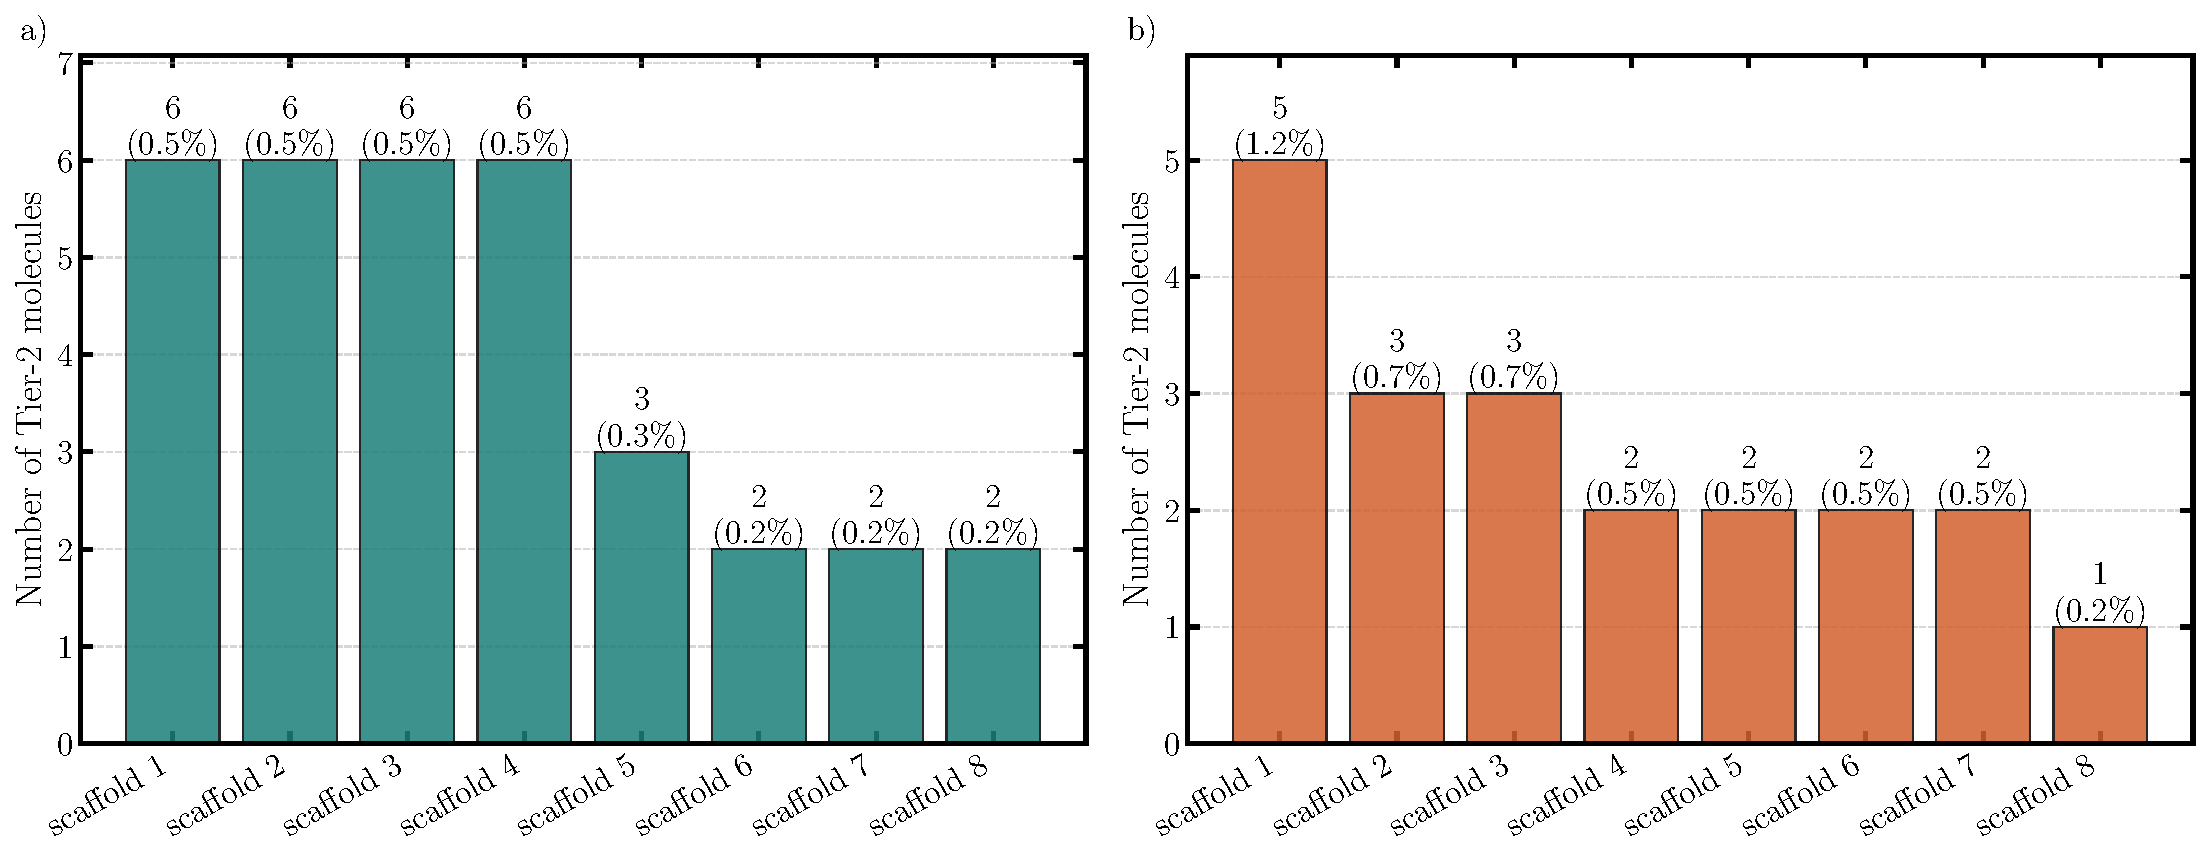
\includegraphics[width=16 cm]{figures/tier2_scaffold_family_bars.pdf}
\caption{(a) Most frequent Bemis--Murcko scaffolds among the unique donor molecules comprising the Tier-2 shortlist, expressed as counts and as a percentage of the corresponding unique-molecule set ($n\_{\mathrm{donor}}=1{,}099$). (b) Most frequent Bemis--Murcko scaffolds among the unique acceptor molecules comprising the Tier-2 shortlist, expressed as counts and as a percentage of the corresponding unique-molecule set ($n\_{\mathrm{acceptor}}=431$). No individual scaffold exceeds $1.2\%$ of either set.}
\label{fig:tier2_scaffold_family_bars}
\end{figure}

\begin{figure}[!htb]
\centering
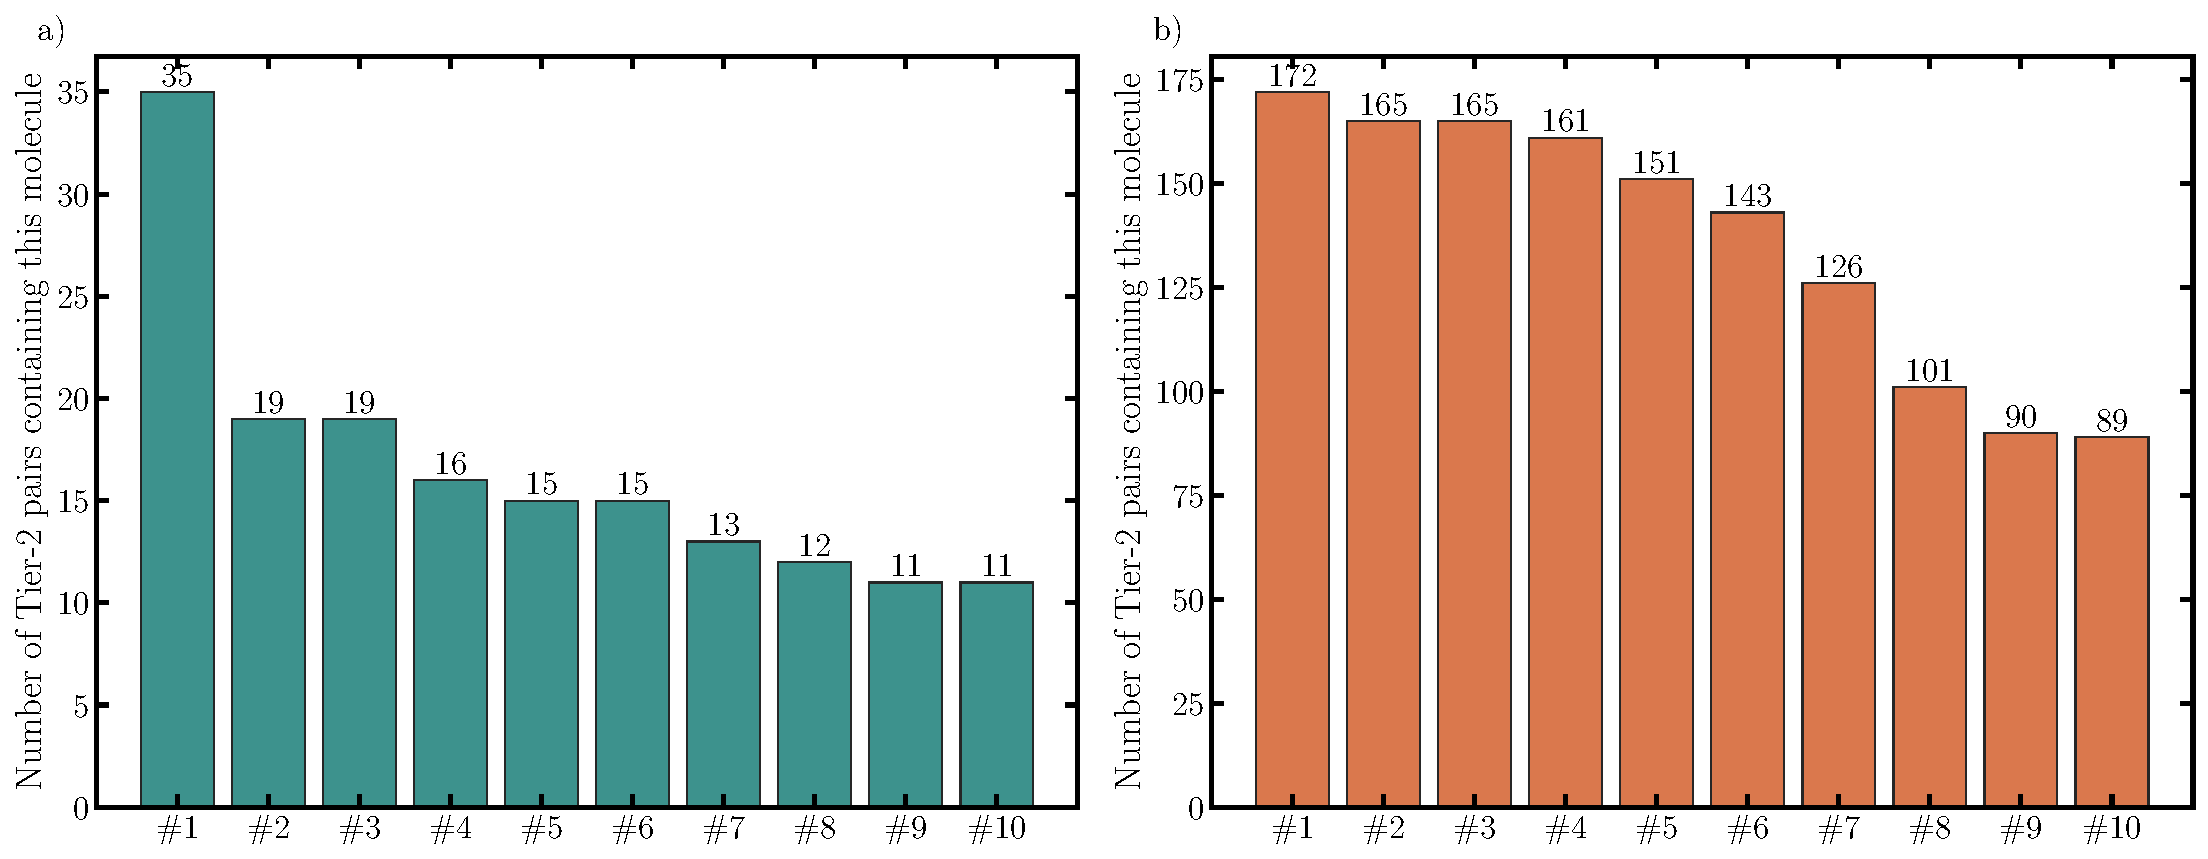
\includegraphics[width=16 cm]{figures/tier2_building_block_recurrence.pdf}
\caption{(a) Recurrence of the ten most frequently occurring donor building blocks within the $2{,}832$-pair Tier-2 shortlist. The ten most recurring donors account for $5.9\%$ of Tier-2 pairs. (b) Recurrence of the ten most frequently occurring acceptor building blocks within the $2{,}832$-pair Tier-2 shortlist. The ten most recurring acceptors account for $48.1\%$ of Tier-2 pairs, showing that Tier-2 performance is broadly distributed across donor chemical space but concentrated on a comparatively small set of high-scoring acceptor building blocks.}
\label{fig:tier2_building_block_recurrence}
\end{figure}

\begin{figure}[!htb]
\centering
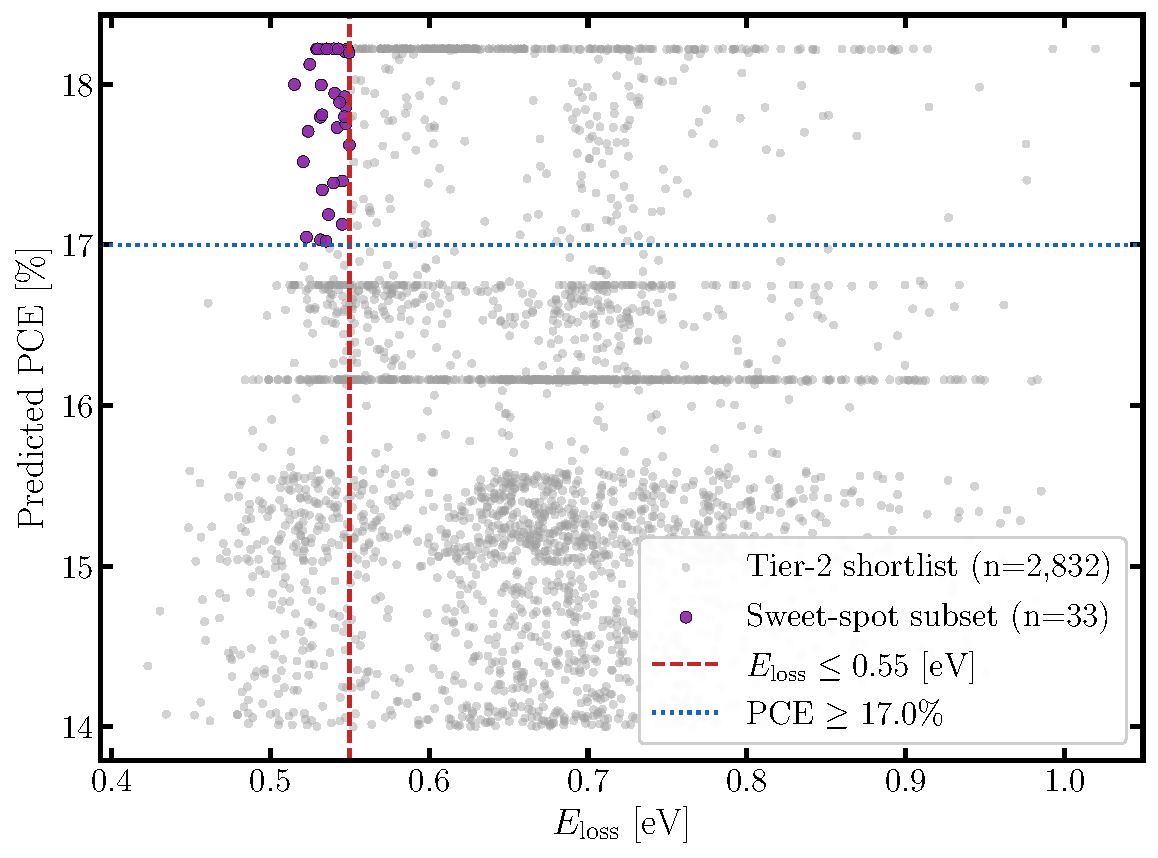
\includegraphics[width=16 cm]{figures/tier2_eloss_pce_sweet_spot.pdf}
\caption{Predicted PCE versus physically screened $E_{\mathrm{loss}}$ for the $2{,}832$ Tier-2 pairs (grey), with the $33$ pairs jointly satisfying $E_{\mathrm{loss}}\le0.55$~eV and $\mathrm{PCE}\ge17.0\%$ highlighted (purple). The sweet-spot candidates are concentrated around a small number of recurring acceptor building blocks rather than being distributed uniformly across the shortlist.}
\label{fig:tier2_eloss_pce_sweet_spot}
\end{figure}

\begin{table}[!htb]
\centering
\caption{Summary of molecular-library diversity, synthetic-accessibility screening, device-relevant prioritisation, and validation outcomes for generated donor and acceptor candidates. Pair-level quantities are reported across the combined donor--acceptor set.}
\label{tab:consolidated_metrics}
\scriptsize
\setlength{\tabcolsep}{3pt}
\begin{tabular}{lcc}
\hline
\textbf{Metric} & \textbf{Donor} & \textbf{Acceptor} \\
\hline
\multicolumn{3}{l}{\textit{Library composition}} \\
Unique generated molecules, $n$ & 52{,}995 & 53{,}719 \\
Reference molecules in FP--PCA--FD baseline$^{a}$ & 157 & 481 \\
\hline
\multicolumn{3}{l}{\textit{Structural diversity and novelty}} \\
MOSES mean-pairwise internal diversity, $\mathrm{IntDiv} = 1-\langle T_{ij}\rangle$ & 0.848 & 0.813 \\
Bemis--Murcko scaffold diversity & 0.768 & 0.824 \\
Unique scaffolds & 40{,}701 & 44{,}282 \\
Nearest-neighbour similarity, $\overline{S_{\mathrm{NN}}}$ & 0.171 & 0.199 \\
Fraction with $S_{\mathrm{NN}} < 0.5$ & 97.0\% & 99.9\% \\
\hline
\multicolumn{3}{l}{\textit{Chemical-space comparison}} \\
Fingerprint-space distance & 25.23 & 16.97 \\
Property-embedding distance & 444.3 & 428.0 \\
ChemNet distance & 26.51 & n/a$^{b}$ \\
Descriptor-distribution agreement & 0.919 & 0.642 \\
Normalized 1-Wasserstein distance, $\overline{W}_1$ & 1.564 & 2.192 \\
Mean Mahalanobis distance & 448 & 1787 \\
\hline
\multicolumn{3}{l}{\textit{Synthetic accessibility}} \\
Mean synthetic-accessibility score & 3.91 & 3.64 \\
Mean retrosynthesis-feasibility score & 0.674 & 0.776 \\
Candidates meeting combined accessibility criteria & 85.0\% & 99.3\% \\
Mean building-block compatibility score & 0.463 & 0.502 \\
\hline
\multicolumn{3}{l}{\textit{Structure-disjoint predictive reliability ($R^2$)}} \\
Frontier-orbital properties & $-0.33$ to $-0.25$$^{c}$ & $+0.44$ to $+0.69$$^{d}$ \\
\hline
\multicolumn{3}{l}{\textit{Pair-level screening across $n=11{,}988{,}459$ donor--acceptor pairs}} \\
Predicted PCE, mean (maximum) & \multicolumn{2}{c}{5.87\% (18.22\%)} \\
Predicted $J_{sc}$, mean (maximum) & \multicolumn{2}{c}{11.28 (27.70) mA cm$^{-2}$} \\
Predicted $FF$, mean (maximum) & \multicolumn{2}{c}{0.534 (0.785)} \\
Predicted $V_{oc}$, mean (maximum) & \multicolumn{2}{c}{0.854 (1.295) V} \\
Structure-disjoint $R^2$: PCE / $J_{sc}$ / $FF$ / $V_{oc}$ & \multicolumn{2}{c}{0.11--0.41 / $-0.10$--0.39 / $-1.04$--$-0.57$ / $-0.78$--$+0.38$$^{e}$} \\
Prioritised donor--acceptor pairs & \multicolumn{2}{c}{2{,}832} \\
\hline
\multicolumn{3}{l}{\textit{Generative-model balance}} \\
Final discriminator / generator loss & 0.671 / 0.668 & 0.676 / 0.649 \\
Final discriminator accuracy & 53.2\% & 51.9\% \\
Training epochs & 5 & 5 \\
\hline
\multicolumn{3}{l}{\textit{Retrosynthesis assessment of prioritised structures}} \\
Structures classified as accessible & \multicolumn{2}{c}{$n=864$; 76.5\%} \\
\hline
\end{tabular}
\par\vspace{3pt}
\parbox{\textwidth}{\scriptsize
$^{a}$Counts denote unique molecules after pooling the DMPNN and Guzik reference libraries for the FP--PCA--FD split-half baseline; they are not the 300 paired device records used to train the screening surrogate.
$^{b}$The ChemNet distance was not available for the acceptor set because the sampled molecular strings exceeded the encoder-length limit.
$^{c}$The donor reference space is too small and structurally limited for reliable structure-disjoint extrapolation.
$^{d}$The acceptor frontier-orbital estimates show useful, but not definitive, structure-disjoint transferability.
$^{e}$The $V_{oc}$ range spans a negative held-out $R^2$ under donor-disjoint ($-0.73$) and scaffold-disjoint ($-0.78$) evaluation but a positive value under acceptor-disjoint evaluation ($+0.38$); $V_{oc}$ transferability is therefore protocol dependent rather than uniformly negative (Section~3.5.1).}
\end{table}


\clearpage
\bibliographystyle{achemso}
\bibliography{references}
\end{document}